\documentclass[
11pt,%
tightenlines,%
twoside,%
onecolumn,%
nofloats,%
nobibnotes,%
nofootinbib,%
superscriptaddress,%
noshowpacs,%
centertags]%
{revtex4}
\usepackage{ljm}
\usepackage{listings}
\usepackage[utf8]{inputenc}
\usepackage[russian]{babel}

\lstset{
language=C++,
basewidth=0.5em,
xleftmargin=45pt,
xrightmargin=45pt,
basicstyle=\small\ttfamily,
keywordstyle=\bfseries\underbar,
numbers=left,
numberstyle=\tiny,
stepnumber=1,
numbersep=10pt,
showspaces=false,
showstringspaces=false,
showtabs=false,
frame=trBL,
tabsize=2,
captionpos=t,
breaklines=true,
breakatwhitespace=false,
escapeinside={\%*}{*)}
}

\begin{document}

\titlerunning{Computational mesh evolution}
\authorrunning{Meshcheryakov et al.}

\title{Evolution of the surface computational mesh in the ice accretion process}

\author{\firstname{A.~O.}~\surname{Meshcheryakov}}
\email[E-mail: ]{alex2501@jscc.ru}
\affiliation{Joint Supercomputer Center of the Russian Academy of Sciences -- branch of Scientific Research Institute of System Analysis of the Russian Academy of Sciences, Leninsky prospect 32a, Moscow, 119334, Russia}

\author{\firstname{A.~A.}~\surname{Rybakov}}
\email[E-mail: ]{rybakov@jscc.ru}
\affiliation{Joint Supercomputer Center of the Russian Academy of Sciences -- branch of Scientific Research Institute of System Analysis of the Russian Academy of Sciences, Leninsky prospect 32a, Moscow, 119334, Russia}

\firstcollaboration{(Submitted by TODO)} % Add if you know submitter.
%\lastcollaboration{ }

\received{TODO}

\begin{abstract}
Задача моделирования обледенения поверхности обтекаемого тела является критической для обеспечения безопасности полетов в условия ледообразования.
Формирование ледяных наростов на несущих частях и элементах силовых установок летальных аппаратов может существенно влиять на летные характеристики.
Сам процесс ледообразования является комплексным.
Для получения качественной картины профиля ледяного нароста необходимо учитывать множество физических процессов, включая динамику газа, теплопроводность, динамику капель, выпадающих на поверхность, течение жидкости по поверхности.
Расчет ледяного покрова должен выполняться итерационно, так как образующийся лед существенно влияет на газодинамические характеристики, которые должны пересчитываться с ростом льда.
Важной частью моделирования является эволюция поверхности тела в процессе ледообразования.
В настоящей статье рассматриваются различные подходы к моделированию эволюции поверхности, предлагается новый алгоритм построения новой поверхности с помощью общей огибающей семейства сфер, центры которых находятся на исходной поверхности.
В процессе эволюции на поверхности могут образовываться различные артефакты и аномалии, из-за которых проведение дальнейших расчетов может стать невозможным.
Для устранения этих препятствий в статье рассматриваются методы адаптации расчетной сетки в процессе эволюции, а также устранения потенциальных самопересечений, препятствующих дальнейшим расчетам.
\end{abstract}

%\subclass{TODO subclass} % Enter 2010 Mathematics Subject Classification.

\keywords{Ледообразование, неструктурированная поверхностная расчетная сетка, эволюция поверхности.}

\maketitle

%---------------------------------------------------------------------------------------------------

\section{Introduction}
Численное моделирование процесса обледенения поверхности тела является сложной мультифизичной задачей, включающей в себя моделирование процессов газовой динамики, теплообмена, течения жидкости, динамики капель в воздушном потоке и других.
Исследование процессов ледообразования имеет важное практическое значение.
В частности характер и интенсивность образования льда на поверхности летательного аппарата критическим образом влияет на его летные характеристики, что напрямую связано с безопасностью полетов TODO.

На сегодняшний день среди зарубежного программного обеспечения для моделирования процесса ледообразования лидером является программный комплекс ANSYS (включая модули FENSAP-ICE, DROP3D, ICE3D) TODO.
В России также активно ведется разработка математических алгоритмов и программного обеспечения по этому направлению.
Можно отметить исследования по разработке модуля iceFoam в составе открытого пакета OpenFOAM TODO.
Среди коммерческих продуктов в последние годы активно развивается пакет IceVision в составе программного комплекса FlowVision TODO, а также решение в составе пакета инженерного анализа ЛОГОС TODO.

Моделирование процесса ледяного покрова осуществляется, как правило, на поверхностной расчетной сетке и состоит из двух основных частей.
Первой частью является вычисление интенсивности нарастания льда в отдельных элементах сетки (это может быть вычисление массы скопившегося льда в каждой ячейке расчетной сетки за единицу времени, либо скорость образования ледяного покрова в узлах сетки, либо другие аналогичные характеристики).
Для выполнения вычисления интенсивности нарастания льда в элементах расчетной сетки существует множество моделей ледообразования TODO, учитывающих разные состояния льда, динамику водяной пленки, тепловые потоки и другие факторы.
Модели ледообразования не рассматриваются в рамках данной работы.
Второй важной составляющей моделирования ледяного нароста является определение изменения поверхности тела после нарастания на ней слоя льда.
В данной статье рассматриваются наиболее известные подходы к моделированию эволюции поверхности обледеневающего тела, а также предлагается новый алгоритм эволюции поверхности, основанный на принципе общей огибающей семейства сфер, центры которых лежат на поверхности, и алгоритм устранения самопересечений сетки, которые могут возникать из-за изменения положения узлов в процессе эволюции.


%---------------------------------------------------------------------------------------------------

\section{Mesh architecture}
\begin{figure}[h]
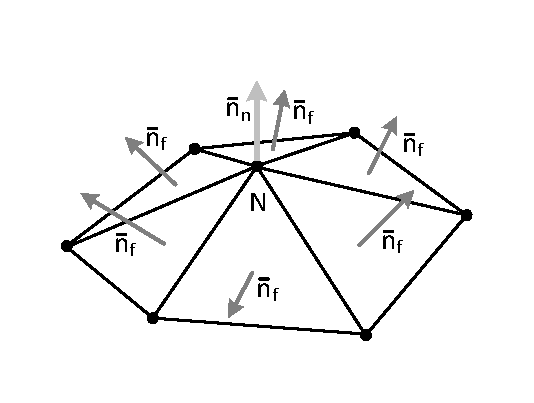
\includegraphics[width=0.48\textwidth]{pics/pic_architecture_size.pdf}
\captionstyle{center}\caption{Архитектура расчетной сетки.}\label{fig:pic_architecture}
\end{figure}


%---------------------------------------------------------------------------------------------------

\section{Remeshing}
Центральная задача перестроения поверхности из-за нарастания ледяного покрова выглядит следующим образом.
Пусть известно, что в результате численного решения задачи ледообразования конечно-объемным методом \cite{Beaugendre} в каждой ячейке сетки была вычислена масса накопленного льда ($m$).
Будем считать плотность льда постоянной, то есть в каждой ячейке также известен объем накопленного льда ($V$).
Для каждого узла сетки $N$ требуется найти его новое положение в пространстве $N'$, чтобы для каждой ячейки с узлами $ABC$ объем пространства, ограниченный фигурой $ABCA'B'C'$ соответствовал объему льда, накопленному в данной ячейке.

Следует отметить, что поставленная задача может не иметь точного решения, и в этом случае следует стремиться к минимизации ошибки по объему (когда фактически образовавшийся объем льда не слишком сильно отличается от целевого объема, то есть разница $V_{ABCA'B'C'} - V$ мала).

Задачу определения новых положений узлов расчетной сетки можно разделить на две задачи: определение направлений смещения узлов и определение величин смещения.
Далее рассмотрим отдельные методы перестроения поверхностей более подробно.

\subsection{Classical remeshing methods}
Простейшие классические методы перестроения выполняются в предположении, что направление смещения узла совпадает с нормалью, проведенной из этого узла.
Таким образом, необходимо лишь определить величину смещения.
Отметим, что в двумерной постановке можно найти оптимальное решение (обеспечивающее минимальное отклонение по объему от целевого значения) поставленной задачи \cite{Rybakov_2D}.

\begin{figure}[h]
  \centering
  \begin{minipage}[h]{0.49\textwidth}
    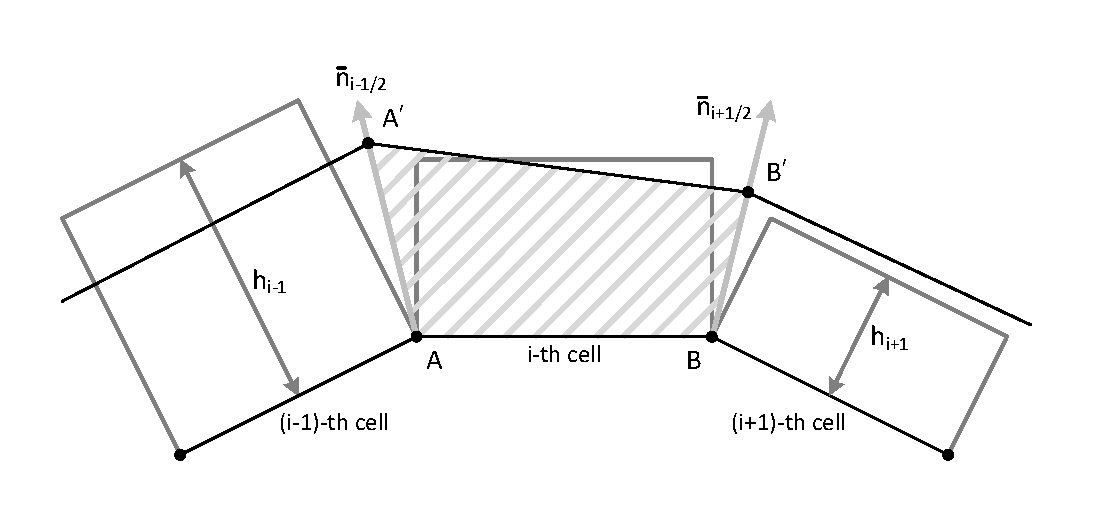
\includegraphics[width=\textwidth]{pics/pic_classical_methods_rectangles_size.pdf}
    \caption{Перестроение поверхности с помощью метода прямоугольников в 2D.}\label{fig:pic_classical_methods_rectangles}
  \end{minipage}
  \hfill
  \begin{minipage}[h]{0.49\textwidth}
    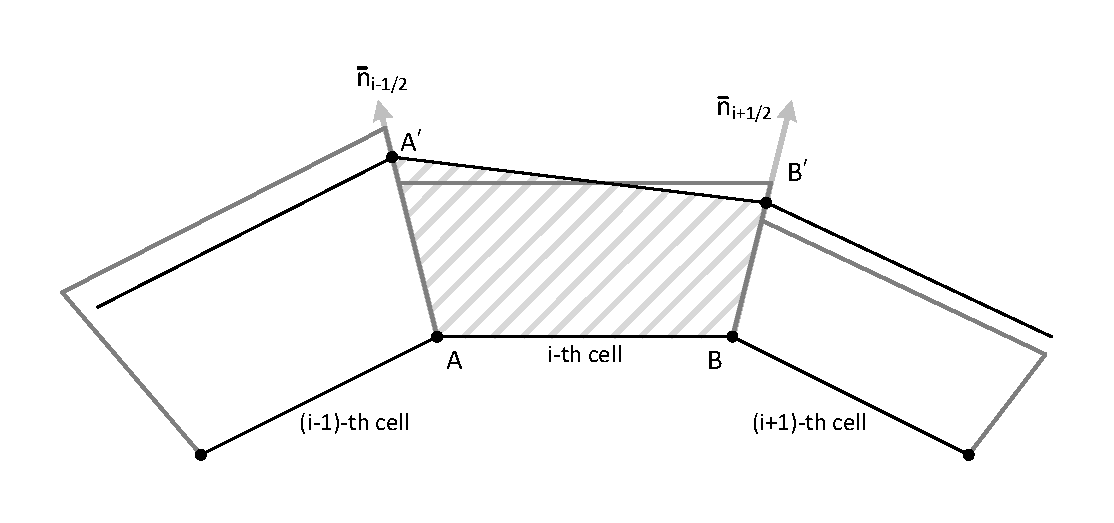
\includegraphics[width=\textwidth]{pics/pic_classical_methods_trapezoids_size.pdf}
    \caption{Перестроение поверхности с помощью метода трапеций в 2D.}\label{fig:pic_classical_methods_trapezoids}
  \end{minipage}
\end{figure}

В качестве первого метода рассмотрим метод призм (в двумерной постановке аналогом данного метода является метод прямоугольников, продемонстрированный на Fig.~\ref{fig:pic_classical_methods_rectangles}).
В этом методе входными данными является объем накопленного льда в каждой ячейке сетки ($V(f)$).
На первым шаге в каждой ячейке ищется толщина ледяного покрова в предположении, что лед в пределах одной ячейки имеет форму призмы, и ячейка является основанием этой призмы.
Тогда толщина ледяного покрова равняется $h(f) = \frac{V(f)}{S(f)}$, где $S(f)$ -- площадь ячейки.
После чего величина смещения каждого узла вычисляется просто как среднее арифметическое высот ледяного покрова во всех инцидентных ячейках:

\begin{equation}
h(N) = \frac{1}{|\mathscr{F}(N)|} \sum_{f \in \mathscr{F}(N)}{h(f)}
\end{equation}

Второй метод можно назвать методом пирамид (в двумерной постановке аналогом данного метод является метод трапеций, показанный на Fig.~\ref{fig:pic_classical_methods_trapezoids}).
Входными данными также является объем накопленного льда в каждой ячейке сетки ($V(f)$).
Однако в отличие от предыдущего метода объем накопленного в ячейке льда представляется не призмой, а усеченной пирамидой, основанием которой является ячейка, а боковые ребра направлены вдоль нормалей узлов.
Высота этой усеченной пирамиды ищется из соотношения $V(f) = \frac{1}{3} h (2S + hS'_h + \sqrt{S(S + hS'_h)})$, где величина $S'_h$ определяется направлениями нормалей узлов ячейки.
Тогда как узлы ячейки являются точками первого основания построенной пирамиды, точки второго основания представляют собой новые положения узлов, вычисленных относительно рассматриваемой ячейки.
Таким образом, у каждого узла сетки вычисляется несколько новых положений (каждое из которых вычислено относительно своей инцидентной ячейки).
Для двумерного случая получается ровно два таких новых положения (так как в двумерном случае каждый узел имеет ровно две инцидентные ячейки), для трехмерного случае таких точек более двух.
Для выбора единственного нового положения узла сетки берется среднее значение из всех положений, вычисленных относительно инцидентных ячеек.

Из рассмотренных двух методов интуитивно создается впечатление, что метод пирамид должен быть более точным, так как он учитывает потери и избыток объема льда, образующиеся из-за изломов сетки (так как соседние ячейки не лежат в одной плоскости, то представление льда в ячейках в виде призм неизбежно приводит к образованию пробелов или наложений частей льда в виде призм друг на друга).
Но по крайней мере в двумерном случае это предположение оказывается неверным, так как метод прямоугольников демонстрирует меньшее отклонение от точного решения по сравнению с методом трапеций \cite{Rybakov_2D}.

\begin{figure}[h]
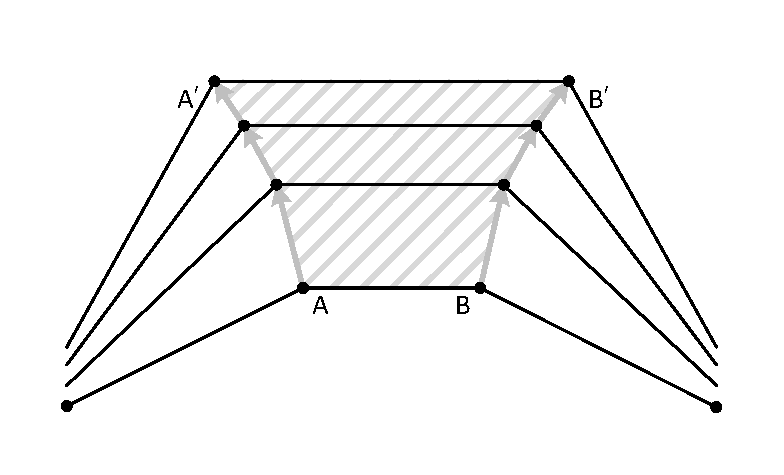
\includegraphics[width=0.48\textwidth]{pics/pic_classical_methods_multilayer_size.pdf}
\captionstyle{center}\caption{Многослойное перестроение сетки.}\label{fig:pic_classical_methods_multilayer}
\end{figure}

Вне зависимости от используемого метода перестроения значительно повысить точность можно с помощью многослойного подхода \cite{BourgaultCote}.
В этом случае вместо однократного перестроения сетки по объему накопленного льда в каждой ячейке ($V(f)$), выбирается фиксированное количество шагов перестроения $k$, а дальше процедура выполняется $k$ раз подряд, но с использованием объема накопленного в ячейке льда $\frac{V(f)}{k}$.
Точность повышается из-за того, что после каждого шага перестроения нормали в узлах сетки меняют свое направление, и общий объем наращиваемого льда становится более криволинейным, лучше учитывает геометрию сетки и, как следствие, точнее соответствует исходному значению $V(f)$ (см. Fig.~\ref{fig:pic_classical_methods_multilayer}).
\subsection{Перестроение сохранением объема}
%В работах \cite{Thompson,Tong} описан устойчивый итерационный алгоритм эволюции поверхностной сетки, сохраняющий целевой объем льда.
The articles \cite{Thompson,Tong} describe a stable iterative grid evolution algorithm that preserves the target volume of ice.
%В нем используется ряд улучшений по сравнению с классическими методами.
It uses several improvements over the classical methods.

%Многослойный подход, реализованный в этом методе, не использует константное количество шагов - величина наращиваемого объема на каждом шаге алгоритма рассчитывается исходя из максимально допустимой доли временного шага обледенения, после превышения которого возможно развитие численной нестабильности в эволюции поверхности.
The multilayer approach implemented in this method does not use a constant number of steps - the value of the increased volume at each step of the algorithm is calculated based on the maximum allowable fraction of the icing time step, after exceeding which numerical instability may occur in the evolution of the surface.
%Наиболее очевидный случай возникает, когда проекции нормалей граней пересекаются, в этом случае слишком большой временной шаг приведет к складыванию поверхности.
The most obvious case occurs when the face normal projections intersect, in which case too large a time step will cause the surface to fold.
%Чтобы идентифицировать грани, которые будут демонстрировать подобное поведение на текущем временном шаге, предполагается, что объем, образованный путем вытягивания треугольной грани с использованием параллельной плоскости смещения, образует призматоид, объем которого определяется кубической функцией высоты $h$:
In order to identify faces that will exhibit such behavior at the current time step, it is assumed that the volume formed by extruding a triangular face using a parallel displacement plane forms a prismatoid whose volume is given by the cubic function of the height $h$:

\begin{equation}\label{Tong:1}
V(h)=ah+bh^2+ch^3
\end{equation}

%где константы $a$, $b$, $c$ определяются позициями узлов грани, их нормалей и нормалью грани.
where the constants $a$, $b$, $c$ are determined by the positions of the face nodes, their normals, and the face normal.
%Рассмотрим корни квадратного уравнения, которое получается в результате дифференцирования уравнения \ref{Tong:1}.
Consider the roots of the quadratic equation, which is obtained as a result of differentiation of the equation \ref{Tong:1}.
%Если корни являются положительными вещественными значениями, наименьший положительный корень определяет высоту, на которой достигается максимальный объем, которая обозначается как $V_{max}$, иначе функция монотонна с возрастанием и ограничение на шаг в данной грани не требуется.
If the roots are positive real values, the smallest positive root determines the height at which the maximum volume is reached, which is denoted as $V_{max}$, otherwise the function is monotonic with increasing and no step restriction is required in this face.
%Исходя из этого, можно вычислить максимальную долю временного шага обледенения, которая требуется для обеспечения разумного поведения накопления объема.
From this, it is possible to calculate the maximum fraction of the icing time step that is required to ensure reasonable volume accumulation behavior.
%В дополнение к этому пределу размера шага был введен предел стабильности $\alpha_{jiao}$, который основан на том, как изменяются направления нормалей по мере эволюции поверхности \cite{Jiao}.
In addition to this step size limit, a $\alpha_{jiao}$ stability limit has been introduced, which is based on how normal directions change as the surface evolves \cite{Jiao}.
%Тогда, допустимая доля временного шага для $i$-й грани определяется как
Then, the allowable fraction of the time step for the $i$-th face is defined as

\begin{equation}\label{Tong:2}
\alpha_{\Delta t}^i=
\begin{cases}
min(s_{\Delta t}\frac{V_{max}^i}{V_f},\alpha_{jiao},1), \text{if $V_{max}^i$ exists}, \\
\alpha_{jiao}, \text{if $V_{max}^i$ doesn't exist}
\end{cases}
\end{equation}

%где $s_{\Delta t}$ ($0 < s_{\Delta t} < 1$) -- эмпирически определяемый коэффициент, $V_f$ -- текущий оставшийся объем приращения льда для $i$-й грани.
where $s_{\Delta t}$ ($0 < s_{\Delta t} < 1$) is an empirically determined coefficient, $V_f$ is the current remaining ice increment volume for the $i$-th face.
%Тогда объем, наращенный для текущего шага, равен $\alpha_{\Delta t} V_f$, где $\alpha_{\Delta t}$ представляет собой глобальное минимальное значение для всех граней.
Then the volume built up for the current step is $\alpha_{\Delta t} V_f$, where $\alpha_{\Delta t}$ is the global minimum value for all faces.

%Другой важной особенностью алгоритма является введение первичного и нулевого простанств, описанных в \cite{Jiao_null_space_smooth}.
Another important feature of the algorithm is the introduction of primary and null spaces, described in \cite{Jiao_null_space_smooth}.
%Если эволюционное движение узлов сетки происходит в первичном пространстве, то их перемещение в нулевом пространстве будет сохранять потенциальную точность второго порядка триангуляции поверхности, благодаря чему мы можем  проводить сглаживание поверхности сетки с сохранением объема.
If the evolutionary movement of mesh nodes occurs in primary space, then their movement in zero space will preserve the potential accuracy of the second order of triangulation of the surface, so that we can maintain volume when smoothing the mesh surface.
%В алгоритме используется несколько видов сглаживаний.
The algorithm uses several types of smoothing.

%Первое сглаживание -- сглаживание нормалей в вершинах и ячейках сетки.
The first smoothing is the smoothing of the normals in the mesh nodes and faces.
%Чтобы сделать возможным сглаживание в нулевом пространстве, все нормали в узлах рассчитываются так, чтобы они лежали в первичном пространстве, а перемещение узлов при наращивании льда происходит только по их нормалям.
To make smoothing possible in zero space, all normals at nodes are calculated so that they lie in primary space, and the movement of nodes during ice buildup occurs only along their normals.
%По мере эволюции, на поверхности может усиливаться шум -- если его не контролировать, может возникнуть ситуация, когда двугранный угол между гранями станет слишком малым и ограничит максимальную долю временного шага обледенения.
As evolution progresses, surface noise can increase - if left unchecked, a situation can arise where the dihedral angle between the faces becomes too small and limits the maximum fraction of the icing time step.
%Для уменьшения поверхностного шума, перед наращиванием льда применяется локальное сглаживание, регулирующее направление смещения узла в проблемных областях, чтобы оно более точно совпадало с направлениями его соседей.
To reduce surface noise, local smoothing is applied before ice builds up, adjusting the direction of node displacement in problem areas so that it more closely matches the directions of its neighbors.
%Этот метод может улучшить гладкость поверхности в некоторых ситуациях.
This method can improve surface smoothness in some situations.
%Основная цель сглаживания нормалей -— вытолкнуть точки из вогнутых областей, где нормали могут локально сходиться.
The main purpose of normal smoothing is to push points out of concave areas where normals can converge locally.
%Сглаживание нормалей достигается с помощью серий взвешенных средних, которые предназначены для придания веса нормалям, генерируемым проблемными областями.
Normal smoothing is achieved using a series of weighted averages, which are designed to give weight to the normals generated by problem areas.

%Второе сглаживание -- сглаживание высот.
The second smoothing is height smoothing.
%После вычисления доли временного шага и объема, наращиваемого для текущего шага, для эволюции поверхности необходимо определить поле высот, которое будет соответствовать этому объему, чтобы по нему определить смещения узлов сетки.
After calculating the fraction of the time step and the volume that is increased for the current step, it is necessary to determine the height field for the evolution of the surface , which will correspond to this volume, in order to determine the offsets of the grid nodes from it.
%Решение $V(h_i) = \alpha_{\Delta t} V_f$ обеспечивает поле начальных высот, которое используется для движения поверхности.
The solution $V(h_i) = \alpha_{\Delta t} V_f$ provides the initial height field that is used to move the surface.
%Цель дополнительного шага сглаживания высоты состоит в том, чтобы отфильтровать высокочастотный шум в поле высот за счет уменьшения разницы высот между соседними гранями.
The purpose of the additional height smoothing step is to filter out high-frequency noise in the height field by reducing the difference in height between adjacent faces.
%Как правило, высоты двух треугольных граней, имеющих общее ребро, не будут равными.
Usually, the heights of two triangular faces that share a common edge will not be equal.
%На данном шаге используется сглаживание высот с сохранением объема путем его перераспределения между соседними гранями.
At this step, smoothing of heights is used while preserving the volume by redistributing it between adjacent faces.

\begin{figure}
  \centering
  \begin{minipage}[h]{0.49\textwidth}
    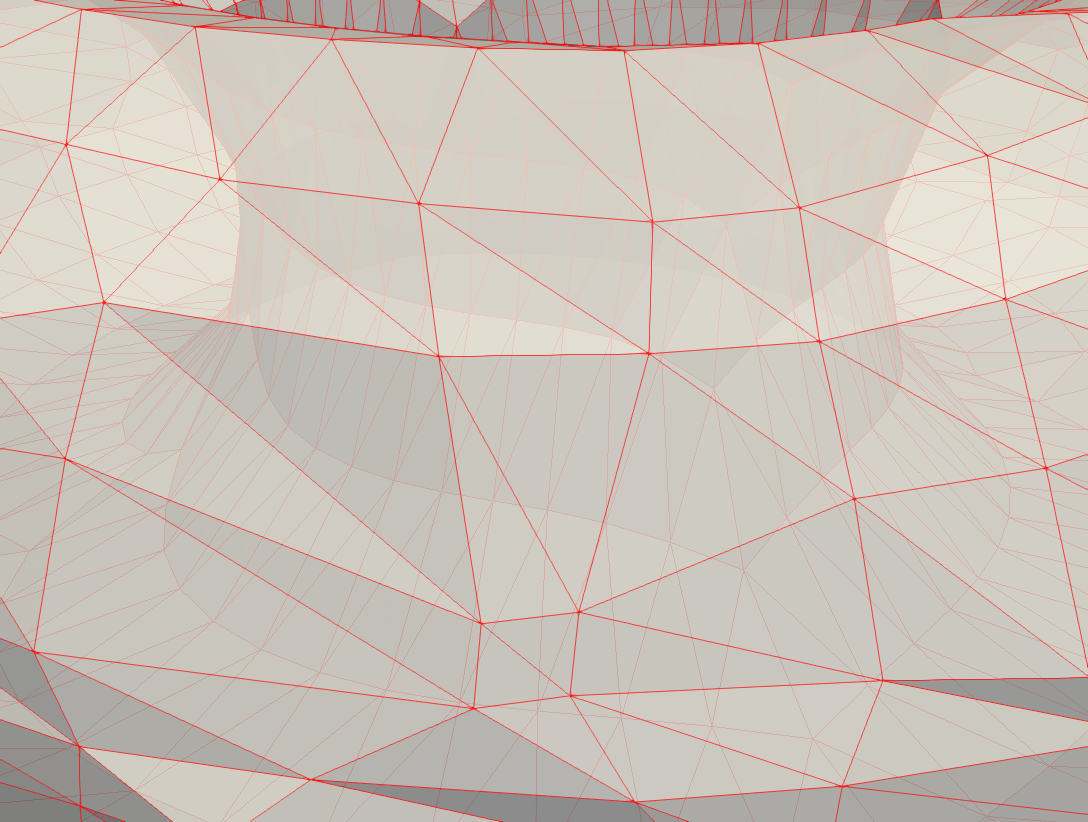
\includegraphics[width=\textwidth]{pics/pic_smooth_before.png}
    \caption{Mesh before null-space smoothing}\label{fig:pic_smooth_before}
  \end{minipage}
  \hfill
  \begin{minipage}[h]{0.49\textwidth}
    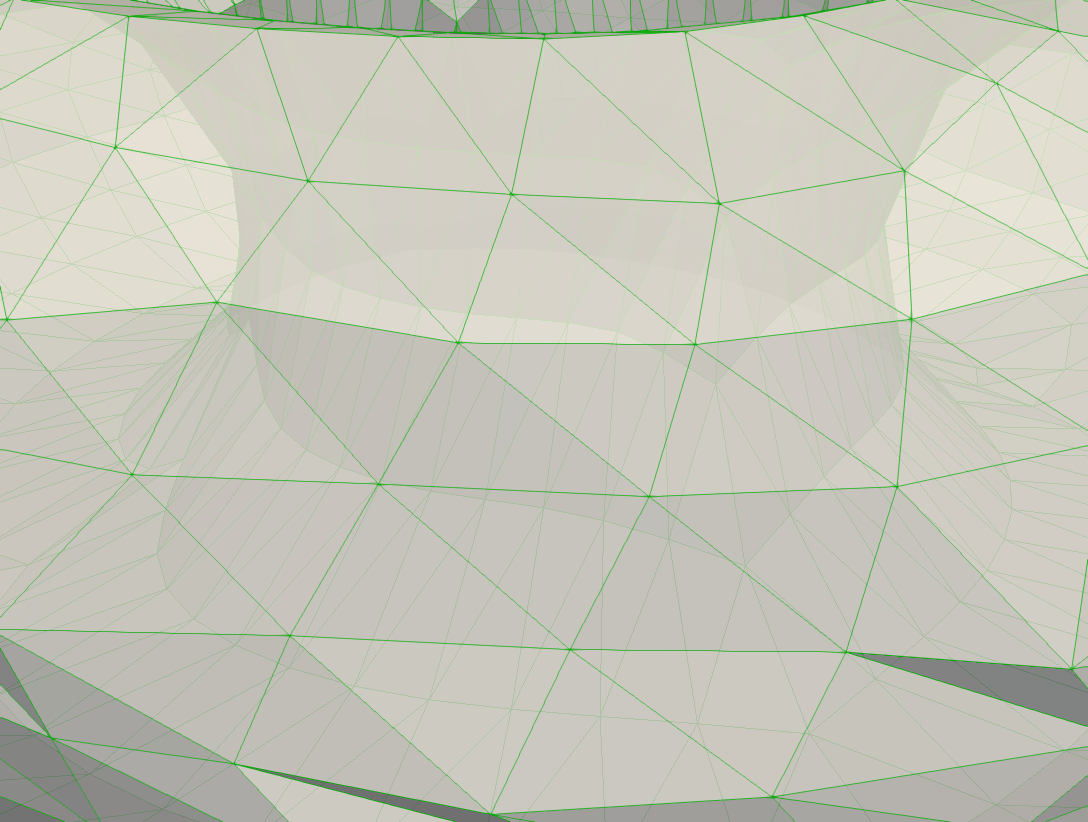
\includegraphics[width=\textwidth]{pics/pic_smooth_after.png}
    \caption{Mesh after null-space smoothing.}\label{fig:pic_smooth_after}
  \end{minipage}
\end{figure}

%Последним типом сглаживания является сглаживание в нулевом пространстве.
The last type of smoothing is null space smoothing.
%Эволюция поверхности будет стремиться упаковать узлы в вогнутые области, где сходятся нормали к поверхности, тогда как расширение сетки происходит в выпуклых областях, где нормали к поверхности расходятся.
Surface evolution will tend to pack nodes into concave regions where surface normals converge, while mesh expansion occurs in convex regions where surface normals diverge.
%Если узлы не будут перераспределены, может стать невозможным продолжать продуктивный, стабильный временной шаг.
If the nodes are not reallocated, it may become impossible to continue with a productive and stable time step.
%Для улучшения качества поверхностной сетки узлы перераспределяются на поверхности с помощью сглаживания в нулевом пространстве.
To improve the quality of the surface mesh, the nodes are redistributed on the surface using null space smoothing.
%Этот метод способен перераспределять точки, сохраняя при этом целостность базовой геометрии.
This method is able to redistribute points while maintaining the integrity of the base geometry.
%Нулевое пространство определяется касательной плоскостью (для гладких областей), касательной линией (для складок поверхности) или пустым пространством (для углов), движущиеся в нем узлы остаются на поверхности, так что объем и форма поверхности могут быть сохранены (Fig.~\ref{fig:pic_smooth_before}, Fig.~\ref{fig:pic_smooth_after}).
Null space is defined by a tangent plane (for smooth areas), a tangent line (for surface wrinkles), or empty space (for corners), nodes moving in it remain on the surface, so that the volume and shape of the surface can be preserved (Fig.~\ref{fig:pic_smooth_before}, Fig.~\ref{fig:pic_smooth_after}).
\subsection{Метод общей огибающей}
Перестроение -- огибающая

%---------------------------------------------------------------------------------------------------

\section{Adaptation}
Все рассмотренные в предыдущем разделе методы перестроения поверхностей объединяет одно сходство -- они сохраняют количество элементов расчетной сетки (узлы, ребра, грани) и связи между ними.
Несмотря на некоторые специальные методы по предотвращению конфликтов между гранями сетки и методы сглаживания, после формирования новой поверхности возможно возникновение самопересечений, появление граней неправильной формы, а также неравномерное распределение граней в сетке по размеру.
Пока опустим самопересечения сетки и будем рассматривать только вопросы, касающиеся формы и размера ячеек.

\begin{figure}[h]
  \centering
  \begin{minipage}[h]{0.35\textwidth}
    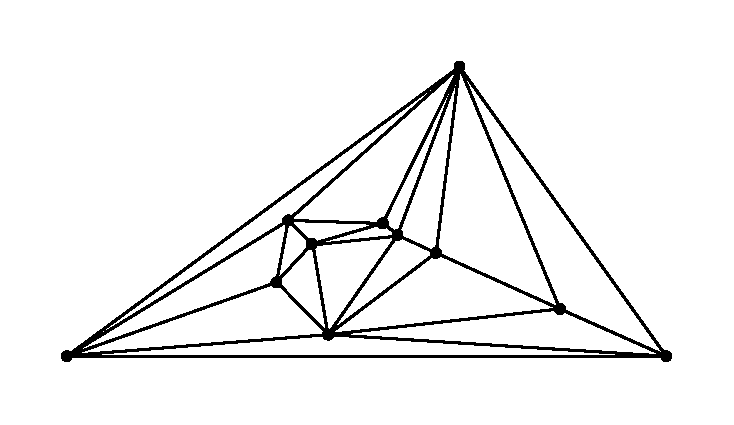
\includegraphics[width=\textwidth]{pics/pic_delaunay_size.pdf}
    \caption{Разбиение ячейки с помощью триангуляции Делоне.}\label{fig:pic_delaunay}
  \end{minipage}
  \hfill
  \begin{minipage}[h]{0.35\textwidth}
    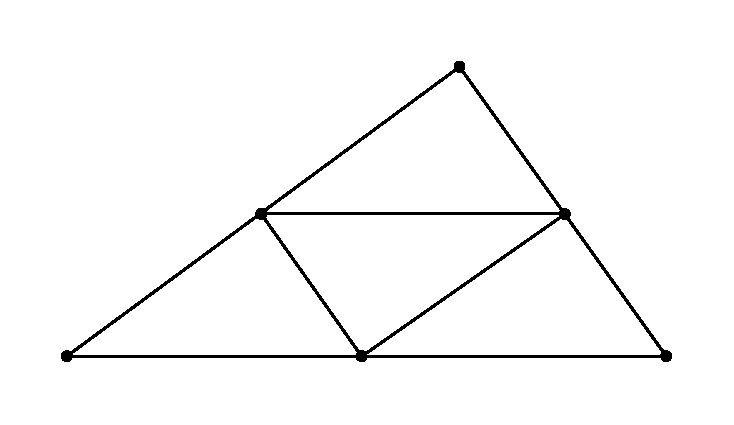
\includegraphics[width=\textwidth]{pics/pic_delaunay_2_size.pdf}
    \caption{Дробление ячейки на более мелкие.}\label{fig:pic_delaunay_2}
  \end{minipage}
  \hfill
  \begin{minipage}[h]{0.28\textwidth}
    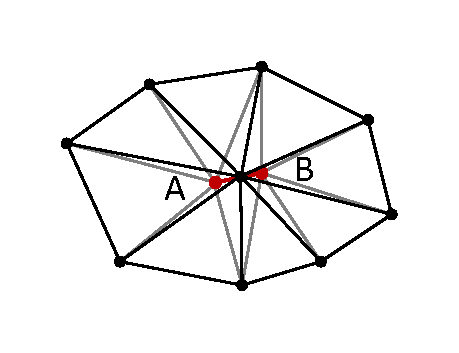
\includegraphics[width=\textwidth]{pics/pic_reduce_edge_size.pdf}
    \caption{Стягивание ребра.}\label{fig:pic_reduce_edge}
  \end{minipage}
\end{figure}

Первая операция, которая нам потребуется -- разбиение ячейки на более мелкие.
Во всех случаях будем выполнять разбиение ячеек с помощью триангуляции Делоне, считая что для разбиения нам известен набор точек внутри разбиваемой ячейки (Fig.~\ref{fig:pic_delaunay}) \cite{Rivara}.
Стоит отметить, что разбиение ячейки можно производить с сохранением локальной кривизны сетки, как это показано в \cite{Rakotoarivelo}, но для простоты будем производить разбиение исключительно в плоскости ячейки.
Если точка разбиения находится не внутри ячейки, а на ее ребре, то разбить придется также вторую инцидентную ячейку этого ребра (рассматриваются только сетки, ребра которых имеют ровно по две инцидентные ячейки, как это указано в (\ref{eq_arch}).
Иногда для уменьшения размера требуется просто разбить ячейку на более мелкие без задания точек разбиения.
В этом случае необходимо следить за качеством результирующих ячеек.
Для определения качества формы ячейки треугольной формы с узлами $\vec{A}$, $\vec{B}$, $\vec{C}$ можно пользоваться простым критерием качества

\begin{equation}
Q(f) = \frac{4\sqrt{3} S_{ABC}}{|\vec{AB}|^2 + |\vec{BC}|^2 + |\vec{AC}|^2}
\end{equation}

где $Q(f) = 1$ соответствует идеальному случаю равносторонней ячейки, а $Q(f) = 0$ -- худший случай для ячеек с нулевой площадью \cite{Borouchaki}.
Для выполнения разбиения ячейки на более мелкие с сохранением их качества просто выполним разбиение по серединам всех ее сторон (Fig.~\ref{fig:pic_delaunay_2}).

Вторая операция, которая необходима для адаптации сетки, связана с огрублением.
Достаточно часто во время выполнения триангуляции по множеству заданных точек могут появляться ячейки с низким показателем качества (у них могут присутствовать либо слишком острые углы, либо близкий к развернутому угол).
Если в ячейке присутствует угол, близкий к развернутому, то избавиться от него поможет разбиение по наибольшей стороне (при этом в качестве точки разбиения следует выбрать основание высоты, опущенной из противолежащего узла).
Если же в треугольнике присутствуют лишь близкие к острым углы, то значит в нем есть слишком короткая сторона, которая может быть удалена.
При удалении ребра $AB$ удаляются обе инцидентные ей грани, узлы $A$ и $B$ соединяются в единый узел $A'$, а все ребра из множества $\mathscr{E}(A) \cup \mathscr{E}(B)$ перенаправляются на узел $A'$ с учетом удаления повторных (Fig.~\ref{fig:pic_reduce_edge}).
Данную операцию будем называть стягиванием ребра \cite{Panchal}.
Путем применения стягивания наиболее коротких ребер в расчетной сетке можно добиться произвольной степени огрубления.


%---------------------------------------------------------------------------------------------------

\section{Устранение самопересечений}
\subsection{Поиск треугольников}
Устранение самопересечений -- поиск треугольников и точек пересечения
\subsection{Zipper}
Устранение самопересечений -- zipper
\subsection{Дробление ячеек}
\begin{figure}
  \centering
  \begin{minipage}[b]{0.49\textwidth}
    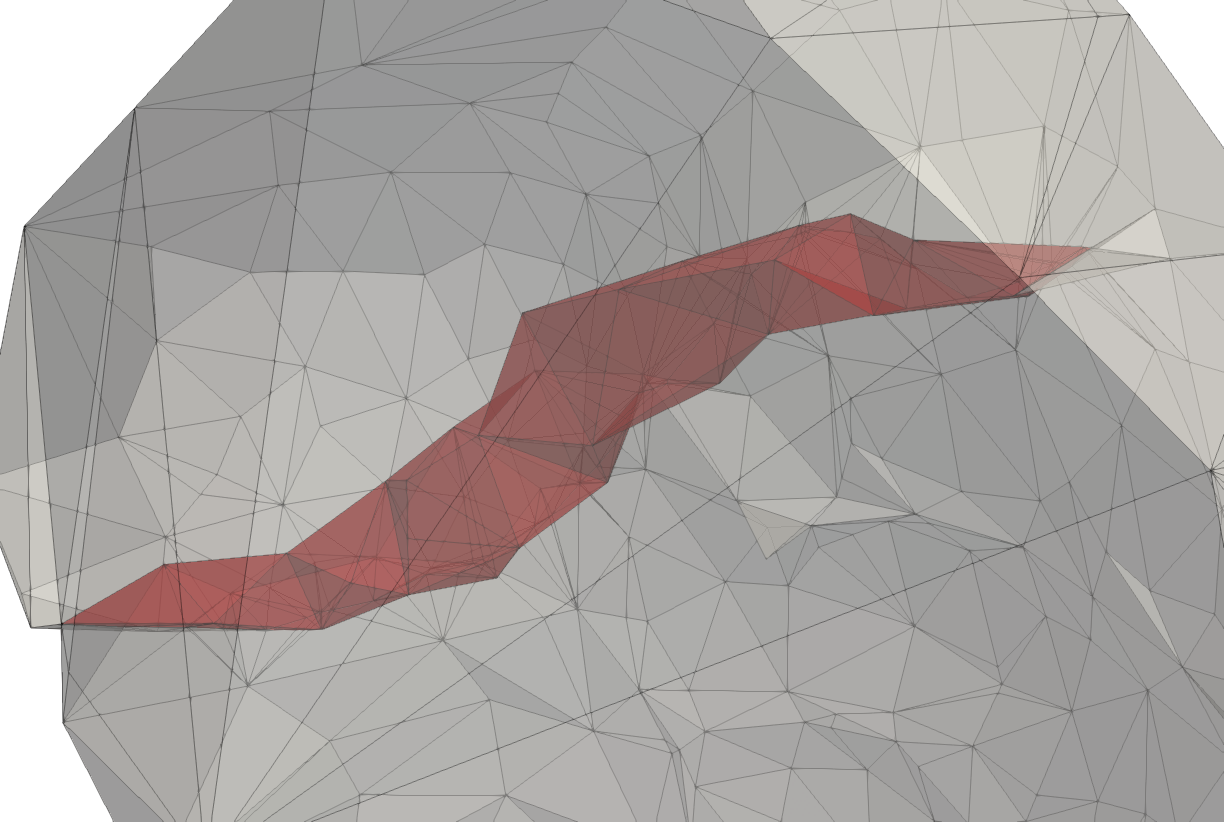
\includegraphics[width=\textwidth]{pics/pic_self_intersection_on.png}
    \caption{Поверхность до удаления самопересечения.}\label{fig:pic_self_intersection_on}
  \end{minipage}
  \hfill
  \begin{minipage}[b]{0.49\textwidth}
    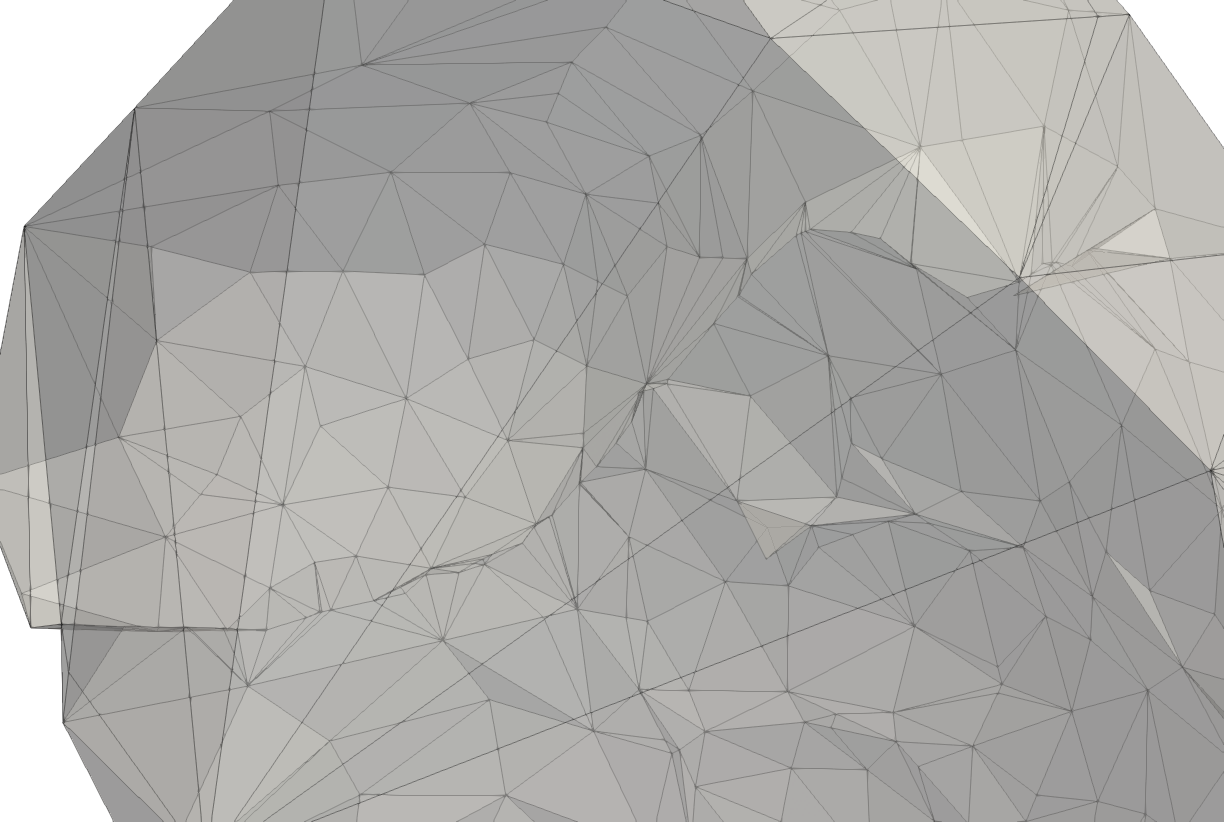
\includegraphics[width=\textwidth]{pics/pic_self_intersection_off.png}
    \caption{Поверхность после удаления самопересечения.}\label{fig:pic_self_intersection_off}
  \end{minipage}
\end{figure}

\begin{figure}
  \centering
  \begin{minipage}[b]{0.49\textwidth}
    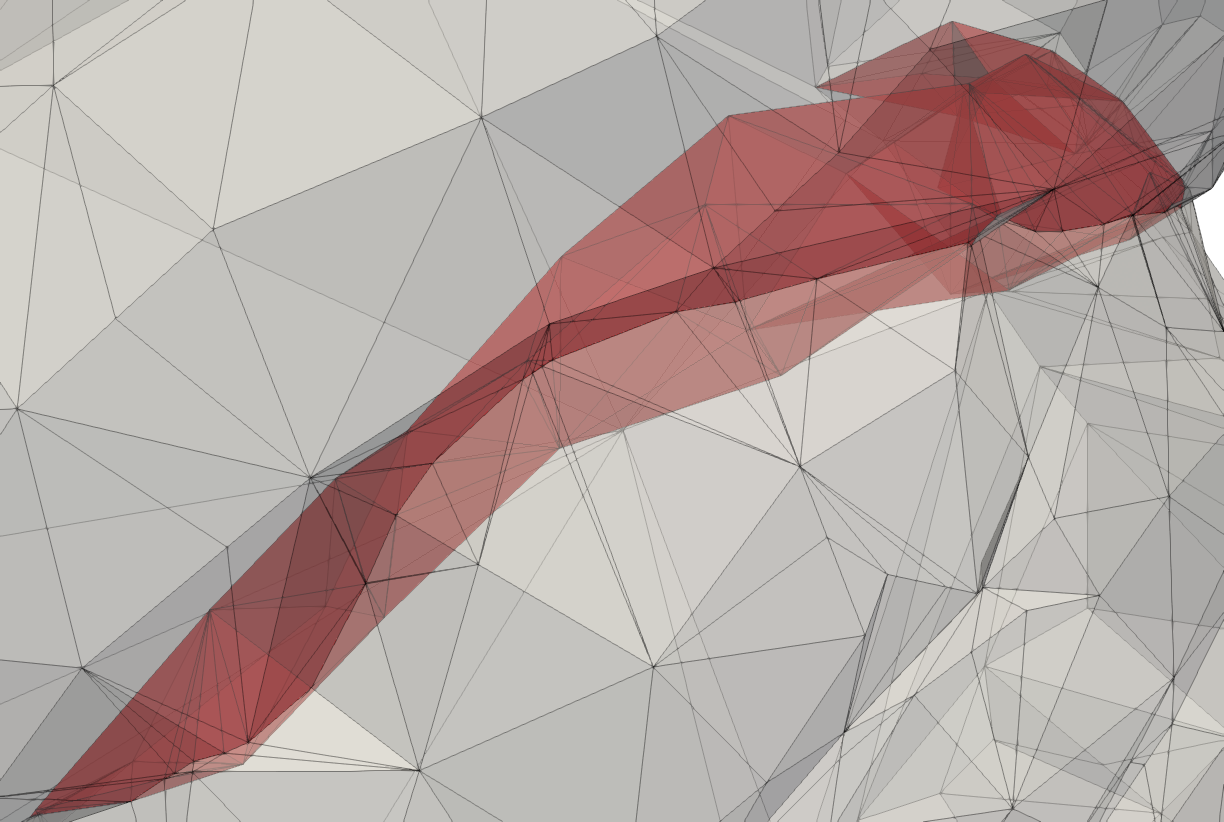
\includegraphics[width=\textwidth]{pics/pic_self_intersection_on_2.png}
    \caption{Поверхность до удаления самопересечения.}\label{fig:pic_self_intersection_on}
  \end{minipage}
  \hfill
  \begin{minipage}[b]{0.49\textwidth}
    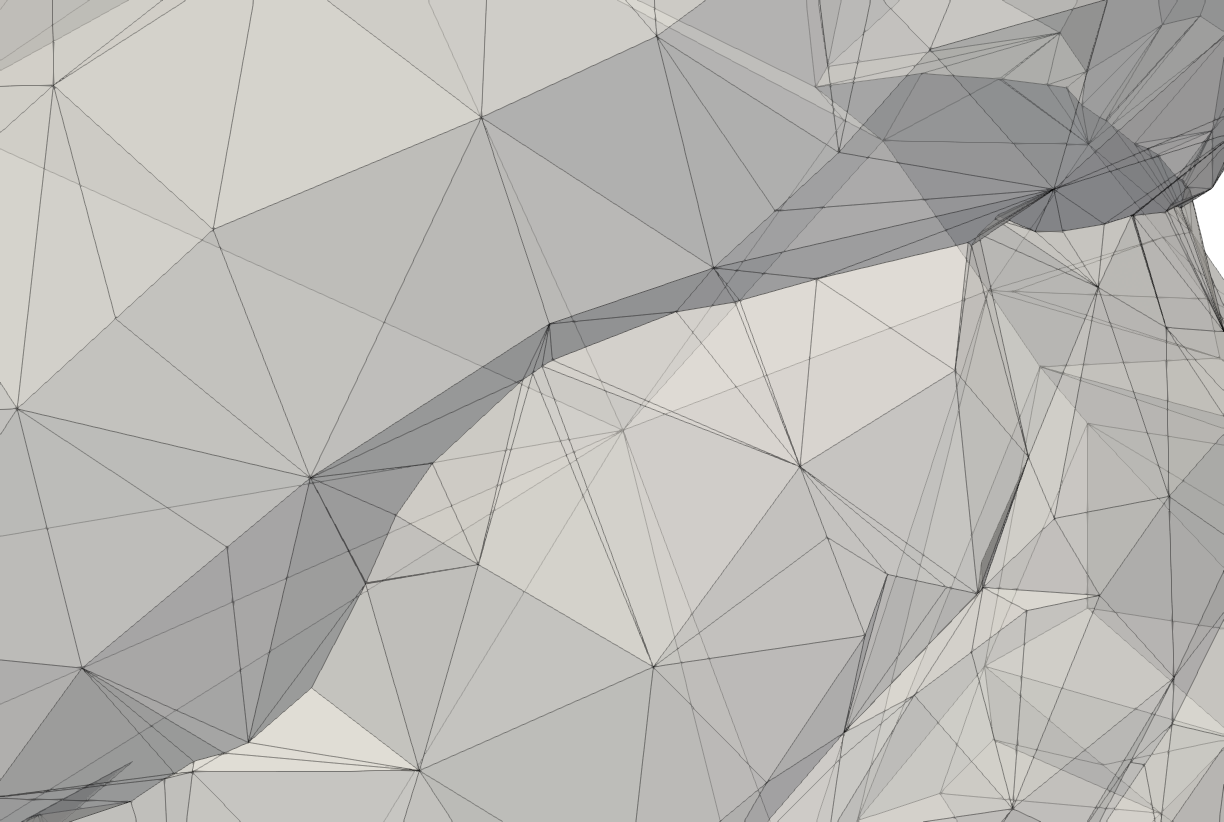
\includegraphics[width=\textwidth]{pics/pic_self_intersection_off_2.png}
    \caption{Поверхность после удаления самопересечения.}\label{fig:pic_self_intersection_off}
  \end{minipage}
\end{figure}

%---------------------------------------------------------------------------------------------------

\section{Conclusion}
It is established the invariance of the structure of the wavelet-fractal-correlation DO type identification algorithm to the peculiarities of the current phono-target environment controlled by OED.

The statistical stability of the initial sufficient statistics for the algorithm and the statistical stability of DO type identification algorithm itself are proved for various features of its flight path and sight.

The performance indicators of the wavelet-fractal-correlation type recognition algorithm are estimated for various real-world operating conditions of the OED as the primary sensor of the sets of measurements of the coordinates of the elevation angle, azimuth and range of the detected DO at each finite current time interval and the stable performance of the algorithm in both simple and complex phono-target conditions for the functioning of the OED, including during intensive maneuvering of DO.

Set forth above it represents the development of the theory of methods for assessing the stability of the functioning of algorithms in the conditions of statistical and tactical uncertainty about the current phono-target situation in the zone of control of OED.


\begin{acknowledgments}
The work was carried out at the JSCC RAS as part of the government assignment (topic FNEF-2022-0016). Supercomputer MVS-10P was used in research.
\end{acknowledgments}

%---------------------------------------------------------------------------------------------------

\begin{thebibliography}{99}

% Introduction.

\bibitem{Raj}
\refitem{article}
L.~Prince Raj, K.~Yee, and R.~S.~Myong, \textquotedblleft Sensivity of ice and aerodynamic performance degradation to critical physical and modeling parameters affecting airfoil icing,\textquotedblright \ Aerospace Science and Technology, {\bf 98}, 105659 (2020).

\bibitem{Martini}
\refitem{article}
F.~Martini, H.~Ibrahim, L.~T.~C.~Montoya, P.~Rizk, and A.~Ilinca, \textquotedblleft Turbulence modeling of iced wind turbine airfoils,\textquotedblright \ Energies, {\bf 15}, 8325 (2022).

\bibitem{Strijhak}
\refitem{article}
S.~Strijhak, V.~Melnikova, and K.~Koshelev, \textquotedblleft Development of iceFoam solver for modeling ice accretion,\textquotedblright \ in \textit{Proceedings of the Institute for System Programming of RAS, 2020}.

\bibitem{Sorokin}
\refitem{article}
K.~E.~Sorokin, P.~M.~Byvaltsev, A.~A.~Aksenov, S.~V.~Zhluktov, D.~V.~Savitskiy, A.~A.~Babulin, and V.~I.~Shevyakov, \textquotedblleft Numerical simulation of ice accretion if FlowVision sotfware,\textquotedblright \ Computer Research and Modeling, {\bf 12}, №~1, 83--96 (2020).

\bibitem{Galanov}
\refitem{article}
N.~G.~Galanov, A.~V.~Sarazov, R.~N.~Zhukov, and A.~S.~Kozelkov, \textquotedblleft Application of various ice accretion simulation approaches in the LOGOS software package,\textquotedblright \ Journal of Physics: Conference Series, {\bf 2099}, 012029 (2021).

\bibitem{Bartkus}
T.~P.~Bartkus, P.~M.~Struk, and J.-C.~Tsao, \textquotedblleft Evaluation of a thermodynamic ice-crystal icing model using experimental ice accretion data,\textquotedblright \ in \textit{Proceedings of the Atmospheric and Space Environments Conference, 2018}

\bibitem{Zhang}
X.~Zhang, X.~Wu, and J.~Min, \textquotedblleft Aircraft icing model considering both rime ice property variability and runback water effect,\textquotedblright \ International Journal of Heat and Mass Transfer, {\bf 104}, 510--516 (2017).

\bibitem{Pena}
D.~Pena, Y.~Hoarau, and E.~Laurendeau, \textquotedblleft A single step ice accretion model using level-set method,\textquotedblright \ Journal of Fluids and Structures, {\bf 65}, 278--294 (2016).


% Remesh.

\bibitem{Beaugendre}
\refitem{misc}
H.~Beaugendre, \textquotedblleft A PDE-based approach to in-flight ice accretion,\textquotedblright \ PhD Thesis (Dep. of Mech. Eng., McGill Univ., Montr\'eal, Qu\'ebec, 2003).

\bibitem{Rybakov_2D}
\refitem{article}
A.~Rybakov and S.~Shumilin, \textquotedblleft Approximate methods of the surface mesh deformation in two-dimensional case,\textquotedblright \ Lobachevskii J Math {\bf 40}, 1848--1852 (2019).

\bibitem{BourgaultCote}
\refitem{article}
S.~Bourgault-C\^ot\'e, K.~Hasanzadeh, P.~Lavoie, and E.~Laurendeau, \textquotedblleft Multi-layer icing methodologies for conservative ice growth,\textquotedblright \ in \textit{Proceedings of 7th European Conference for Aeronautics and Aerospace Sciences EUCASS, 2017}.

\bibitem{Thompson}
\refitem{article}
D.~Thompson, X.~Tong, Q.~Arnoldus, E.~Collins, D.~McLaurin, and E.~Luke, \textquotedblleft Discrete surface evolution and mesh deformation for aircraft icing applications,\textquotedblright \ in \textit{Proceedings of the 5th AIAA Atmospheric and Space Environments Conference, 2013}.

\bibitem{Tong}
\refitem{article}
X.~Tong, D.~Thompson, Q.~Arnoldus, E.~Collins, and E.~Luke, \textquotedblleft Three-dimensional surface evolution and mesh deformation for aircraft icing applications,\textquotedblright \ Journal of Aircraft, {\bf 54}, 1047--1063 (2017).

\bibitem{Jiao}
\refitem{article}
X.~Jiao, \textquotedblleft Face offsetting: a unified approach for explicit moving interfaces,\textquotedblright \ Journal of Computational Physiscs, {\bf 220}, 612--625 (2007).

\bibitem{Jiao_null_space_smooth}
\refitem{article}
X.~Jiao, \textquotedblleft Volume and feature preservation in surface mesh optimization,\textquotedblright \ in \textit{Proceedings of the 15th International Meshing Roundtable, 2006}.

% Adaptation.

\bibitem{Borouchaki}
\refitem{article}
H.~Borouchaki, P.~Laug, and P.-L.~George, \textquotedblleft Parametric surface meshing using a combined advancing-front generalized Delaunay approach,\textquotedblright \ International Journal for Numerical Methods in Engineering, {\bf 49}, 233--259 (2000).

\bibitem{Rivara}
\refitem{article}
M.-C.~Rivara and P.~A.~Rodrigez-Moreno, \textquotedblleft Tuned terminal triangles centroid Delaunay algorithm for quality triangulation,\textquotedblright \ in \textit{27th International Meshing Roundtable, 2019}.

\bibitem{Rakotoarivelo}
\refitem{article}
H.~Rakotoarivelo and F.~Ledoux, \textquotedblleft Accurate manycore-accelerated manifold surface remesh kernels,\textquotedblright \ in \textit{27th International Meshing Roundtable, 2019}.

\bibitem{Panchal}
\refitem{article}
D.~Panchal and D.~Jayaswal, \textquotedblleft Feature sensitive geometrically faithful highly regular direct triangular isotropic surface remeshing,\textquotedblright \ S$\bar{a}$dhan$\bar{a}$, {\bf 47}, 94 (2022).

% SLE

\bibitem{Jung}
\refitem{article}
W.~Jung, H.~Shin, and B.~K.~Choi, \textquotedblleft Self-intersection removal in triangular mesh offsettings,\textquotedblright \ CAD Journal, {\bf 1}, № 1, 477--484 (2004).

\bibitem{Skvorkovska}
\refitem{article}
V.~Skorkovsk\'a, I.~Kolingerov\'a, and B.~Benes, \textquotedblleft A Simple and robust approach to computation of meshes intersection,\textquotedblright \ in \textit{Proceedings of the 13th International Joint Conference on Computer Vision, Imaging and Computer Graphics Theory and Applications, {\bf 1}, 175--182, 2018}.

\bibitem{Charton}
\refitem{article}
J.~Charton, S.~Baek, and Y.~Kim, \textquotedblleft Mesh repairing using topology graphs,\textquotedblright \ Journal of Computational Design and Engineering, {\bf 8}, 251--267 (2021).

\bibitem{Freylekhman}
\refitem{article}
S.~A.~Freylekhman and A.~A.~Rybakov, \textquotedblleft Self-intersection elimination for unstructured surface computational meshes,\textquotedblright \ Lobachevskii J Math {\bf 43}, 134--140 (2022).


\end{thebibliography}

\end{document}
